% !TEX spellcheck = en_US



% ~~~~~~~~~~~~~~~~~~~~~~~~~~~~~~~~~~~~~~~ V
% (NC) 2026 Haluk Bingol
% github.com/halukbingol/LaTeX-Templates
%
% Licensees may copy, distribute, display, and perform the work and make derivative works 
% and remixes based on it only for non-commercial purposes. 
% ~~~~~~~~~~~~~~~~~~~~~~~~~~~~~~~~~~~~~~~ A




% =====================================================================
%  Java on the Command Line -- Junior Level: Modules, Custom Runtimes and Installers
%  ---------------------------------------------------------------------
%  Built on hbCisLaTeXTemplate.tex with the libraries in ../../hblib/.
%  Programs, terminal sessions and their real outputs are in codeoutput/:
%     codeoutput/<Name>.java  a program        codeoutput/<Name>.sh   a session
%     codeoutput/<Name>/      the session's project folder
%     codeoutput/<Name>.txt   what it printed, made by:  bash run_examples.sh
% =====================================================================

\documentclass[aspectratio=169,10pt,compress]{beamer}

% ~~~~~~~~~~~~~~~~~~~~~~~~~~~~~~~~~~~~~~~~~~~~~~~~~~~~~~~~~~~~~~~~~ V hblib
	\usepackage{../../hblib/hblibPresentation} % lib presentation: theme, i/N, \hSection, algorithm2e, ...
	\usepackage{../../hblib/hblibCodeoutput} % lib code + output: \lstcode, \lstterminal, ...
	\usepackage{../../hblib/hblibDatastructures} % lib data structures: \hString, \hStack, \hQueue
% ~~~~~~~~~~~~~~~~~~~~~~~~~~~~~~~~~~~~~~~~~~~~~~~~~~~~~~~~~~~~~~~~~ A hblib


% xcolor, array (and the L{width} column), listings, tikz and algorithm2e come from the hblib libraries
\usepackage[T1]{fontenc}
\usepackage{lmodern}
\usepackage{booktabs}

\definecolor{gitred}{RGB}{240,80,50}
\newcommand{\win}{\textbf{Windows}}
\newcommand{\mac}{\textbf{macOS}}

% ---------------------------------------------------------------------
\title{Java on the Command Line}
\subtitle{Junior Level: Modules, Custom Runtimes and Installers}
\author[Bingol]{Haluk O. Bingol}

\institute[FCIS]{
    Faculty of Computer and Information Sciences\\
    Yeditepe University
}
\date{
	{\tiny \hbTimeStamp}
}

\begin{document}




% ~~~~~~~~~~~~~~~~~~~~~~~~~~~~~~~~~~~~~~ V frm
\begin{frame}[t,fragile]
  \titlepage
\end{frame}
% ~~~~~~~~~~~~~~~~~~~~~~~~~~~~~~~~~~~~~~ A frm




% ~~~~~~~~~~~~~~~~~~~~~~~~~~~~~~~~~~~~~~ V frm
\begin{frame}[t,fragile] \frametitle{Outline}
  \begin{columns}[T]
    \begin{column}{0.48\textwidth}
      \tableofcontents[sections={1-4}, hideallsubsections]
    \end{column}
    \begin{column}{0.48\textwidth}
      \tableofcontents[sections={5-8}, hideallsubsections]
    \end{column}
  \end{columns}
\end{frame}
% ~~~~~~~~~~~~~~~~~~~~~~~~~~~~~~~~~~~~~~ A frm

% ~~~~~~~~~~~~~~~~~~~~~~~~~~~~~~~~~~~~~~ V
\hSection[Modules]{The Module System}{}{}
% ~~~~~~~~~~~~~~~~~~~~~~~~~~~~~~~~~~~~~~ A

% ~~~~~~~~~~~~~~~~~~~~~~~~~~~~~~~~~~~~~~ V
\subsection[Why]{Why modules?}
% ~~~~~~~~~~~~~~~~~~~~~~~~~~~~~~~~~~~~~~ A




% ~~~~~~~~~~~~~~~~~~~~~~~~~~~~~~~~~~~~~~ V frm
\begin{frame}[t,fragile] \frametitle{Problems of the class path}
  \begin{columns}[T]
    \begin{column}{0.52\textwidth}
      The class path is a \textbf{flat list} of folders and JARs:
      \begin{itemize}\small
        \item \textbf{No hiding}: every \texttt{public} class is usable by everyone, even ``internal'' ones.
        \item \textbf{Missing JARs are found late}: \texttt{NoClassDefFoundError} at run time, maybe after hours.
        \item \textbf{Duplicates}: two versions of a class, the first one wins silently.
        \item \textbf{The whole JDK} is always there: about 70 modules, even for ``Hello''.
      \end{itemize}
    \end{column}
    \begin{column}{0.44\textwidth}
      \begin{block}{Module (Java 9, 2017)}
        \small A named group of packages with a \texttt{module-info.java}:
        \begin{itemize}
          \item \texttt{requires}: what it needs
          \item \texttt{exports}: what others may use
        \end{itemize}
        Checked by \texttt{javac} \textbf{and} by \texttt{java} at start-up.
      \end{block}
      \begin{block}{The JDK itself}
        \small \texttt{java.base}, \texttt{java.sql}, \texttt{java.desktop}, \dots{} Every module reads \texttt{java.base}.
      \end{block}
    \end{column}
  \end{columns}
\end{frame}
% ~~~~~~~~~~~~~~~~~~~~~~~~~~~~~~~~~~~~~~ A frm




% ~~~~~~~~~~~~~~~~~~~~~~~~~~~~~~~~~~~~~~ V frm
\begin{frame}[t,fragile] \frametitle{Two modules}
  \begin{center}
  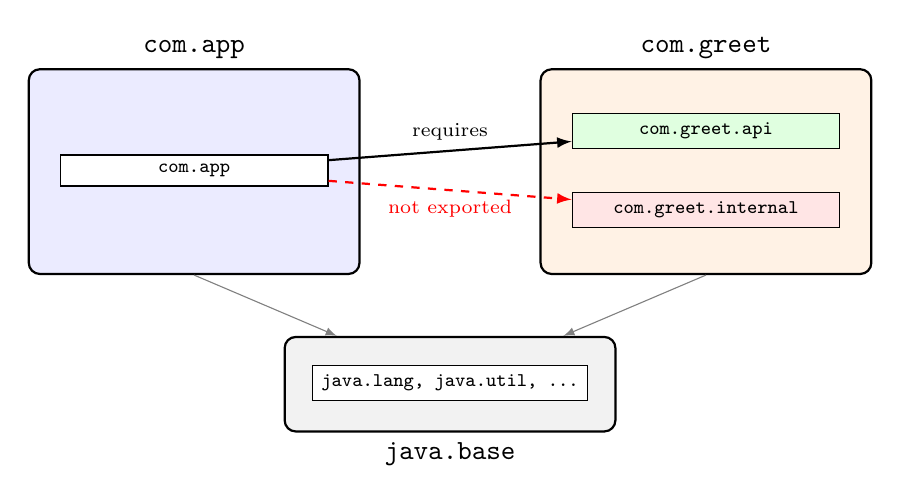
\begin{tikzpicture}[mod/.style={draw, rounded corners, thick, minimum width=4.2cm, minimum height=2.6cm, anchor=north},
                      pkg/.style={draw, fill=white, font=\ttfamily\scriptsize, minimum width=3.4cm}]
    \node[mod, fill=blue!8, label={[font=\ttfamily\bfseries]above:com.app}] (app) at (0,0) {};
    \node[pkg] (m) at (0,-1.3) {com.app};
    \node[mod, fill=orange!10, label={[font=\ttfamily\bfseries]above:com.greet}] (gr) at (6.5,0) {};
    \node[pkg, fill=green!12] (api) at (6.5,-0.8) {com.greet.api};
    \node[pkg, fill=red!10] (int) at (6.5,-1.8) {com.greet.internal};
    \node[mod, minimum height=1.2cm, fill=gray!10, label={[font=\ttfamily\bfseries]below:java.base}] (jb) at (3.25,-3.4) {};
    \node[pkg] at (3.25,-4.0) {java.lang, java.util, \dots};
    \draw[-latex, thick] (m) -- node[above, font=\scriptsize] {requires} (api);
    \draw[-latex, thick, red, dashed] (m) -- node[below, font=\scriptsize] {not exported} (int);
    \draw[-latex, gray] (app.south) -- (jb);
    \draw[-latex, gray] (gr.south) -- (jb);
  \end{tikzpicture}
  \end{center}
  \small Green: exported, usable by \texttt{com.app}. Red: hidden even though \texttt{Words} is \texttt{public}.
  Grey: \texttt{requires java.base} is implicit.
\end{frame}
% ~~~~~~~~~~~~~~~~~~~~~~~~~~~~~~~~~~~~~~ A frm

% ~~~~~~~~~~~~~~~~~~~~~~~~~~~~~~~~~~~~~~ V
\subsection[Project]{A modular project}
% ~~~~~~~~~~~~~~~~~~~~~~~~~~~~~~~~~~~~~~ A




% ~~~~~~~~~~~~~~~~~~~~~~~~~~~~~~~~~~~~~~ V frm
\begin{frame}[t,fragile] \frametitle{The source tree: one folder per module}
  \begin{columns}[T]
    \begin{column}{0.56\textwidth}
      \lstcode[basicstyle=\ttfamily\tiny]{codeoutput/Project/src/com.greet/module-info.java}{Java}
      \lstcode[basicstyle=\ttfamily\tiny]{codeoutput/Project/src/com.app/module-info.java}{Java}
      \lstcode[basicstyle=\ttfamily\tiny]{codeoutput/Project/src/com.app/com/app/Main.java}{Java}
    \end{column}
    \begin{column}{0.42\textwidth}
      \begin{itemize}\small
        \item \texttt{src/com.greet} and \texttt{src/com.app}: one folder per module, named after the module.
        \item Inside it, \texttt{module-info.java} at the top and the packages as folders, as before.
        \item Module names look like package names (reverse domain); the two need not be equal.
      \end{itemize}
    \end{column}
  \end{columns}
\end{frame}
% ~~~~~~~~~~~~~~~~~~~~~~~~~~~~~~~~~~~~~~ A frm




% ~~~~~~~~~~~~~~~~~~~~~~~~~~~~~~~~~~~~~~ V frm
\begin{frame}[t,fragile] \frametitle{The library classes}
  \lstcode[basicstyle=\ttfamily\tiny]{codeoutput/Project/src/com.greet/com/greet/internal/Words.java}{Java}
  \lstcode[basicstyle=\ttfamily\tiny]{codeoutput/Project/src/com.greet/com/greet/api/Greeter.java}{Java}
\end{frame}
% ~~~~~~~~~~~~~~~~~~~~~~~~~~~~~~~~~~~~~~ A frm




% ~~~~~~~~~~~~~~~~~~~~~~~~~~~~~~~~~~~~~~ V frm
\begin{frame}[t,fragile] \frametitle{Compiling and running modules}
  \lstterminal[basicstyle=\ttfamily\tiny]{codeoutput/Modules.txt}

  \vspace{0.1em}
  \small
  \texttt{--module-source-path src} finds every module under \texttt{src}; \texttt{-m} names the modules to compile.
  Run with \texttt{-p} (\texttt{--module-path}) and \texttt{-m module/main.class}. \win: same commands; \texttt{-p} lists use \texttt{;}.
\end{frame}
% ~~~~~~~~~~~~~~~~~~~~~~~~~~~~~~~~~~~~~~ A frm

% ~~~~~~~~~~~~~~~~~~~~~~~~~~~~~~~~~~~~~~ V
\subsection[Resolution]{Resolution}
% ~~~~~~~~~~~~~~~~~~~~~~~~~~~~~~~~~~~~~~ A




% ~~~~~~~~~~~~~~~~~~~~~~~~~~~~~~~~~~~~~~ V frm
\begin{frame}[t,fragile] \frametitle{What \texttt{java -p mods -m com.app} does first}
% +++++++++++++++++++++++++++++++++++++++ V alg
%: -Alg. 
\begin{algorithm}[H]
  \caption{Resolving modules at start-up}
  \KwIn{root module $r$, module path $p$}
  \KwOut{the set $R$ of modules to load, or an error \textbf{before} \texttt{main} runs}
  $R \gets \emptyset$\;
  $Q \gets \langle r, \texttt{java.base} \rangle$\;
  \While{$Q$ is not empty}{
    $m \gets$ \textsc{Dequeue}$(Q)$\;
    \lIf{$m \in R$}{\textbf{continue}}
    \lIf{$m$ is neither in the JDK nor on $p$}{\textbf{fail} \texttt{FindException: Module $m$ not found}}
    $R \gets R \cup \{ m \}$\;
    \ForEach{\texttt{requires} $n$ of $m$}{\textsc{Enqueue}$(Q, n)$\;}
  }
  check: no package in two modules of $R$, no cycles\;
  \Return{$R$}\;
\end{algorithm}
% +++++++++++++++++++++++++++++++++++++++ A alg

\end{frame}
% ~~~~~~~~~~~~~~~~~~~~~~~~~~~~~~~~~~~~~~ A frm

% ~~~~~~~~~~~~~~~~~~~~~~~~~~~~~~~~~~~~~~ V
\subsection[Encapsulation]{Strong encapsulation}
% ~~~~~~~~~~~~~~~~~~~~~~~~~~~~~~~~~~~~~~ A




% ~~~~~~~~~~~~~~~~~~~~~~~~~~~~~~~~~~~~~~ V frm
\begin{frame}[t,fragile] \frametitle{Forgetting \texttt{requires}}
  \lstterminal[basicstyle=\ttfamily\scriptsize]{codeoutput/NoRequires.txt}

  \vspace{0.1em}
  \small Without \texttt{requires com.greet}, module \texttt{com.app} does not \emph{read} \texttt{com.greet}:
  nothing of it is visible, even exported packages.
\end{frame}
% ~~~~~~~~~~~~~~~~~~~~~~~~~~~~~~~~~~~~~~ A frm




% ~~~~~~~~~~~~~~~~~~~~~~~~~~~~~~~~~~~~~~ V frm
\begin{frame}[t,fragile] \frametitle{Using a hidden package}
  \begin{columns}[T]
    \begin{column}{0.36\textwidth}
      \lstcode[basicstyle=\ttfamily\tiny]{codeoutput/Illegal/Main.java}{Java}
    \end{column}
    \begin{column}{0.62\textwidth}
      \uncover<2->{\lstterminal[basicstyle=\ttfamily\tiny]{codeoutput/Encapsulation.txt}}
    \end{column}
  \end{columns}

  \vspace{0.1em}
  \small \texttt{public} is not enough: the package must be \textbf{exported}. \texttt{--add-exports}
  (and \texttt{--add-opens} for reflection) break the rule on purpose, at compile \emph{and} at run time: a last resort for old code.
\end{frame}
% ~~~~~~~~~~~~~~~~~~~~~~~~~~~~~~~~~~~~~~ A frm

% ~~~~~~~~~~~~~~~~~~~~~~~~~~~~~~~~~~~~~~ V
\hSection[Modular JARs]{Modular JARs}{}{}
% ~~~~~~~~~~~~~~~~~~~~~~~~~~~~~~~~~~~~~~ A




% ~~~~~~~~~~~~~~~~~~~~~~~~~~~~~~~~~~~~~~ V frm
\begin{frame}[t,fragile] \frametitle{A modular JAR = a JAR with \texttt{module-info.class}}
  \lstterminal[basicstyle=\ttfamily\tiny]{codeoutput/ModJar.txt}

  \vspace{0.1em}
  \small
  The same JAR works on the \textbf{module path} (\texttt{-p}, checked) and on the \textbf{class path} (\texttt{-cp},
  \texttt{module-info} ignored). A plain JAR on \texttt{-p} becomes an \emph{automatic module} named after the file.
\end{frame}
% ~~~~~~~~~~~~~~~~~~~~~~~~~~~~~~~~~~~~~~ A frm




% ~~~~~~~~~~~~~~~~~~~~~~~~~~~~~~~~~~~~~~ V frm
\begin{frame}[t,fragile] \frametitle{Class path or module path?}
  \begin{center}\small
  \begin{tabular}{lll}
    \toprule
                         & class path \texttt{-cp}            & module path \texttt{-p} \\
    \midrule
    unit                 & folders, JARs                     & modules (modular or automatic JARs) \\
    missing dependency   & \texttt{NoClassDefFoundError}, late & \texttt{FindException}, at start-up \\
    two copies           & first one wins                    & error \\
    hidden packages      & none                              & everything not \texttt{exports}ed \\
    run                  & \texttt{java -cp a.jar p.Main}    & \texttt{java -p mlib -m mod/p.Main} \\
    custom runtime       & no                                & \texttt{jlink} \\
    \bottomrule
  \end{tabular}
  \end{center}
  \vspace{0.5em}
  \small Most libraries are still used on the class path; new applications benefit from modules mostly when they want \texttt{jlink}.
\end{frame}
% ~~~~~~~~~~~~~~~~~~~~~~~~~~~~~~~~~~~~~~ A frm

% ~~~~~~~~~~~~~~~~~~~~~~~~~~~~~~~~~~~~~~ V
\hSection[jlink]{Custom Runtimes: jlink}{}{}
% ~~~~~~~~~~~~~~~~~~~~~~~~~~~~~~~~~~~~~~ A




% ~~~~~~~~~~~~~~~~~~~~~~~~~~~~~~~~~~~~~~ V frm
\begin{frame}[t,fragile] \frametitle{A runtime with only the modules we need}
  \lstterminal[basicstyle=\ttfamily\tiny]{codeoutput/Jlink.txt}

  \vspace{0.1em}
  \small
  \texttt{jdeps --print-module-deps} tells which JDK modules are needed. The image has its own \texttt{bin/java} and a
  \texttt{hello} launcher; it does \textbf{not} need an installed JDK. Compare its size with an image of all of Java SE (\texttt{--compress zip-6} makes both smaller).
\end{frame}
% ~~~~~~~~~~~~~~~~~~~~~~~~~~~~~~~~~~~~~~ A frm




% ~~~~~~~~~~~~~~~~~~~~~~~~~~~~~~~~~~~~~~ V frm
\begin{frame}[t,fragile] \frametitle{jlink on Windows and macOS}
  \begin{columns}[T]
    \begin{column}{0.48\textwidth}
      \begin{block}{Windows (Command Prompt)}


% +++++++++++++++++++++++++++++++++++++++ V lst
%: -Lst.
\begin{lstlisting}[style=codesnippet, language={}, basicstyle=\ttfamily\scriptsize]
jlink --module-path mlib ^
      --add-modules com.app ^
      --launcher hello=com.app ^
      --strip-debug --no-header-files ^
      --no-man-pages --output image
image\bin\hello
\end{lstlisting}
% +++++++++++++++++++++++++++++++++++++++ A lst


      \end{block}
    \end{column}
    \begin{column}{0.48\textwidth}
      \begin{block}{macOS (Terminal)}


% +++++++++++++++++++++++++++++++++++++++ V lst
%: -Lst.
\begin{lstlisting}[style=codesnippet, language=bash, basicstyle=\ttfamily\scriptsize]
jlink --module-path mlib \
      --add-modules com.app \
      --launcher hello=com.app \
      --strip-debug --no-header-files \
      --no-man-pages --output image
image/bin/hello
\end{lstlisting}
% +++++++++++++++++++++++++++++++++++++++ A lst


      \end{block}
    \end{column}
  \end{columns}

  \vspace{0.3em}
  \begin{itemize}\small
    \item The image is made for \textbf{one} operating system and CPU: build it on Windows for Windows, on macOS for macOS
      (Apple silicon \texttt{aarch64} and Intel \texttt{x64} differ).
    \item \texttt{jlink} needs the JDK's \texttt{jmods}; it only accepts modules, so every JAR must be modular.
  \end{itemize}
\end{frame}
% ~~~~~~~~~~~~~~~~~~~~~~~~~~~~~~~~~~~~~~ A frm

% ~~~~~~~~~~~~~~~~~~~~~~~~~~~~~~~~~~~~~~ V
\hSection[jpackage]{Installers: jpackage}{}{}
% ~~~~~~~~~~~~~~~~~~~~~~~~~~~~~~~~~~~~~~ A




% ~~~~~~~~~~~~~~~~~~~~~~~~~~~~~~~~~~~~~~ V frm
\begin{frame}[t,fragile] \frametitle{An application folder with a native launcher}
  \lstterminal[basicstyle=\ttfamily\scriptsize]{codeoutput/Jpackage.txt}

  \vspace{0.1em}
  \small
  \texttt{jpackage} runs \texttt{jlink} for us, adds a native launcher (\texttt{bin/Hello}) and puts the JARs into \texttt{lib/app}.
  \texttt{--type app-image} works everywhere; the other types make a real installer.
\end{frame}
% ~~~~~~~~~~~~~~~~~~~~~~~~~~~~~~~~~~~~~~ A frm




% ~~~~~~~~~~~~~~~~~~~~~~~~~~~~~~~~~~~~~~ V frm
\begin{frame}[t,fragile] \frametitle{Installers for Windows and macOS}
  \begin{columns}[T]
    \begin{column}{0.48\textwidth}
      \begin{block}{Windows (Command Prompt)}


% +++++++++++++++++++++++++++++++++++++++ V lst
%: -Lst.
\begin{lstlisting}[style=codesnippet, language={}, basicstyle=\ttfamily\scriptsize]
jpackage --type msi --name Hello ^
  --module-path mlib --module com.app ^
  --win-menu --win-shortcut
rem -> Hello-1.0.msi  (also: --type exe)
\end{lstlisting}
% +++++++++++++++++++++++++++++++++++++++ A lst


      \end{block}
    \end{column}
    \begin{column}{0.48\textwidth}
      \begin{block}{macOS (Terminal)}


% +++++++++++++++++++++++++++++++++++++++ V lst
%: -Lst.
\begin{lstlisting}[style=codesnippet, language=bash, basicstyle=\ttfamily\scriptsize]
jpackage --type dmg --name Hello \
  --module-path mlib --module com.app
# -> Hello-1.0.dmg  (also: --type pkg)
# signing: --mac-sign ...
\end{lstlisting}
% +++++++++++++++++++++++++++++++++++++++ A lst


      \end{block}
    \end{column}
  \end{columns}

  \vspace{0.3em}
  \begin{itemize}\small
    \item \win: \texttt{msi}/\texttt{exe} need the free \textbf{WiX Toolset} on the \texttt{PATH}. Installs into \texttt{C:\textbackslash Program Files\textbackslash Hello}.
    \item \mac: the \texttt{.dmg} contains \texttt{Hello.app}. Unsigned apps are blocked by Gatekeeper; for others to run it, sign and notarize it with an Apple Developer ID.
    \item Linux: \texttt{--type deb} or \texttt{rpm}. There is \textbf{no cross-packaging}: run \texttt{jpackage} on each target system (often in CI).
  \end{itemize}
\end{frame}
% ~~~~~~~~~~~~~~~~~~~~~~~~~~~~~~~~~~~~~~ A frm




% ~~~~~~~~~~~~~~~~~~~~~~~~~~~~~~~~~~~~~~ V frm
\begin{frame}[t,fragile] \frametitle{Which way to ship?}
  \begin{center}\small
  \begin{tabular}{llll}
    \toprule
    deliver                   & user needs          & size     & made with \\
    \midrule
    JAR (+ \texttt{lib/})     & a Java runtime      & KB       & \texttt{jar} \\
    fat JAR                   & a Java runtime      & KB--MB   & \texttt{jar}, Maven Shade \\
    runtime image             & nothing             & 30--60 MB & \texttt{jlink} \\
    app image / installer     & nothing             & 40--70 MB & \texttt{jpackage} \\
    container image           & Docker / Podman     & 100+ MB  & \texttt{Dockerfile} (senior deck) \\
    \bottomrule
  \end{tabular}
  \end{center}
  \small Libraries are shipped as JARs (to Maven Central); desktop applications as installers; services as containers.
\end{frame}
% ~~~~~~~~~~~~~~~~~~~~~~~~~~~~~~~~~~~~~~ A frm

% ~~~~~~~~~~~~~~~~~~~~~~~~~~~~~~~~~~~~~~ V
\hSection[MR JAR]{Multi-Release JARs}{}{}
% ~~~~~~~~~~~~~~~~~~~~~~~~~~~~~~~~~~~~~~ A




% ~~~~~~~~~~~~~~~~~~~~~~~~~~~~~~~~~~~~~~ V frm
\begin{frame}[t,fragile] \frametitle{One JAR, different code for different Java versions}
  \lstterminal[basicstyle=\ttfamily\tiny]{codeoutput/MRJar.txt}

  \vspace{0.1em}
  \small
  Classes under \texttt{META-INF/versions/17/} replace the root ones on Java 17 and newer; Java 8--16 use the root
  classes. \texttt{jar --release 17} puts them there and writes \texttt{Multi-Release: true} into the manifest.
\end{frame}
% ~~~~~~~~~~~~~~~~~~~~~~~~~~~~~~~~~~~~~~ A frm

% ~~~~~~~~~~~~~~~~~~~~~~~~~~~~~~~~~~~~~~ V
\hSection[JVM options]{Tuning the JVM from the Command Line}{}{}
% ~~~~~~~~~~~~~~~~~~~~~~~~~~~~~~~~~~~~~~ A




% ~~~~~~~~~~~~~~~~~~~~~~~~~~~~~~~~~~~~~~ V frm
\begin{frame}[t,fragile] \frametitle{Kinds of options}
  \begin{center}\scriptsize
  \begin{tabular}{lll}
    \toprule
    kind           & example                                & note \\
    \midrule
    standard       & \texttt{-cp}, \texttt{-p}, \texttt{-D}, \texttt{-ea}, \texttt{-version} & stable, \texttt{java --help} \\
    extra \texttt{-X} & \texttt{-Xmx512m}, \texttt{-Xss1m}, \texttt{-Xlog:gc}  & \texttt{java -X} \\
    advanced \texttt{-XX:} & \texttt{-XX:+UseZGC}, \texttt{-XX:+HeapDumpOnOutOfMemoryError} & may change between versions \\
    environment    & \texttt{JDK\_JAVA\_OPTIONS}             & added to every \texttt{java} command \\
    \bottomrule
  \end{tabular}
  \end{center}
  \vspace{0.3em}
  \begin{itemize}\small
    \item \texttt{-Xms}/\texttt{-Xmx}: initial/maximum heap. Default maximum: \(\frac{1}{4}\) of the physical memory.
    \item Options go \textbf{before} the class or \texttt{-jar} file; everything after it is an argument of \texttt{main}.
    \item \win: \texttt{set JDK\_JAVA\_OPTIONS=-Xmx512m}; \mac: \texttt{export JDK\_JAVA\_OPTIONS=-Xmx512m}.
  \end{itemize}
\end{frame}
% ~~~~~~~~~~~~~~~~~~~~~~~~~~~~~~~~~~~~~~ A frm




% ~~~~~~~~~~~~~~~~~~~~~~~~~~~~~~~~~~~~~~ V frm
\begin{frame}[t,fragile] \frametitle{Heap size in practice}
  \begin{columns}[T]
    \begin{column}{0.4\textwidth}
      \lstcode[basicstyle=\ttfamily\tiny]{codeoutput/JvmOptions/Hog.java}{Java}
    \end{column}
    \begin{column}{0.58\textwidth}
      \uncover<2->{\lstterminal[basicstyle=\ttfamily\tiny]{codeoutput/JvmOptions.txt}}
    \end{column}
  \end{columns}

  \vspace{0.1em}
  \small \texttt{JDK\_JAVA\_OPTIONS} is announced with \texttt{NOTE: Picked up \dots} so you know it was used.
  With a 32\,MB heap the program fails quickly with \texttt{OutOfMemoryError}.
\end{frame}
% ~~~~~~~~~~~~~~~~~~~~~~~~~~~~~~~~~~~~~~ A frm

% ~~~~~~~~~~~~~~~~~~~~~~~~~~~~~~~~~~~~~~ V
\subsection[Monitoring]{Looking at a running JVM}
% ~~~~~~~~~~~~~~~~~~~~~~~~~~~~~~~~~~~~~~ A




% ~~~~~~~~~~~~~~~~~~~~~~~~~~~~~~~~~~~~~~ V frm
\begin{frame}[t,fragile] \frametitle{\texttt{jps} and \texttt{jcmd}}
  \begin{columns}[T]
    \begin{column}{0.4\textwidth}
      \lstcode[basicstyle=\ttfamily\tiny]{codeoutput/Monitor/Server.java}{Java}
    \end{column}
    \begin{column}{0.58\textwidth}
      \uncover<2->{\lstterminal[basicstyle=\ttfamily\tiny]{codeoutput/Monitor.txt}}
    \end{column}
  \end{columns}

  \vspace{0.1em}
  \small \texttt{jps} lists running JVMs with their process id; \texttt{jcmd <pid or main class> <command>} asks
  one of them for information (\texttt{jcmd Server help} lists the commands). The same tools work on Windows and macOS.
\end{frame}
% ~~~~~~~~~~~~~~~~~~~~~~~~~~~~~~~~~~~~~~ A frm

% ~~~~~~~~~~~~~~~~~~~~~~~~~~~~~~~~~~~~~~ V
\hSection[Build tools]{Build Tools and Modules}{}{}
% ~~~~~~~~~~~~~~~~~~~~~~~~~~~~~~~~~~~~~~ A




% ~~~~~~~~~~~~~~~~~~~~~~~~~~~~~~~~~~~~~~ V frm
\begin{frame}[t,fragile] \frametitle{Maven and Gradle with modules}
  \begin{columns}[T]
    \begin{column}{0.48\textwidth}
      \begin{block}{Maven: \texttt{mvn package}}


% +++++++++++++++++++++++++++++++++++++++ V lst
%: -Lst.
\begin{lstlisting}[style=codesnippet, language=bash, basicstyle=\ttfamily\tiny]
src/main/java/module-info.java
src/main/java/com/app/Main.java
# the compiler plugin sees module-info and
# puts the dependencies on the module path
mvn package
java -p target/app.jar:libs -m com.app
\end{lstlisting}
% +++++++++++++++++++++++++++++++++++++++ A lst


      \end{block}
    \end{column}
    \begin{column}{0.48\textwidth}
      \begin{block}{Gradle: \texttt{build.gradle.kts}}


% +++++++++++++++++++++++++++++++++++++++ V lst
%: -Lst.
\begin{lstlisting}[style=codesnippet, language=Java, basicstyle=\ttfamily\tiny]
plugins { application }
application {
    mainModule = "com.app"
    mainClass  = "com.app.Main"
}
// ./gradlew run   or   ./gradlew installDist
\end{lstlisting}
% +++++++++++++++++++++++++++++++++++++++ A lst


      \end{block}
    \end{column}
  \end{columns}
  \small \hRemark{Not run here} (they need the internet). Plugins such as \texttt{org.beryx.jlink} or
  \texttt{maven-jlink-plugin} call \texttt{jlink} and \texttt{jpackage} for you; the options are the ones on these slides.
\end{frame}
% ~~~~~~~~~~~~~~~~~~~~~~~~~~~~~~~~~~~~~~ A frm

% ~~~~~~~~~~~~~~~~~~~~~~~~~~~~~~~~~~~~~~ V
\hSection[Summary]{Summary}{}{}
% ~~~~~~~~~~~~~~~~~~~~~~~~~~~~~~~~~~~~~~ A




% ~~~~~~~~~~~~~~~~~~~~~~~~~~~~~~~~~~~~~~ V frm
\begin{frame}[t,fragile] \frametitle{Recipes}
  \begin{center}\scriptsize
  \begin{tabular}{ll}
    \toprule
    goal & command (\win: \texttt{;} in paths, \texttt{\textasciicircum} to continue a line) \\
    \midrule
    compile modules          & \texttt{javac -d mods --module-source-path src -m a,b} \\
    run a module             & \texttt{java -p mods -m b/b.Main} \\
    describe a module        & \texttt{java -p mods --describe-module a} \\
    modular JAR              & \texttt{jar --create --file mlib/b.jar --main-class b.Main -C mods/b .} \\
    needed JDK modules       & \texttt{jdeps --print-module-deps --module-path mlib mlib/b.jar} \\
    custom runtime           & \texttt{jlink -p mlib --add-modules b --launcher b=b --output image} \\
    installer                & \texttt{jpackage --type msi|dmg|deb --name B -p mlib -m b} \\
    multi-release JAR        & \texttt{jar --create --file x.jar -C classes . --release 17 -C c17 .} \\
    heap and options         & \texttt{java -Xmx512m -XshowSettings:vm \dots}, \texttt{JDK\_JAVA\_OPTIONS} \\
    running JVMs             & \texttt{jps}, \texttt{jcmd <pid> VM.flags} \\
    \bottomrule
  \end{tabular}
  \end{center}
\end{frame}
% ~~~~~~~~~~~~~~~~~~~~~~~~~~~~~~~~~~~~~~ A frm




% ~~~~~~~~~~~~~~~~~~~~~~~~~~~~~~~~~~~~~~ V frm
\begin{frame}[t,fragile] \frametitle{Exercises}
  \begin{enumerate}\small
    \item Turn the sophomore project (\texttt{util} + \texttt{books}) into two modules. Which packages must be exported?
    \item Remove \texttt{exports} from \texttt{com.greet} and read the error. Then fix it with \texttt{--add-exports} only on the command line.
    \item Make a \texttt{jlink} image of the books application. How big is it? Does it start faster than \texttt{java -jar}? (\texttt{time})
    \item Build an installer with \texttt{jpackage} on your own laptop (\texttt{msi} on Windows, \texttt{dmg} on macOS) and install it.
    \item Write a multi-release JAR whose Java 21 version uses a \texttt{switch} with patterns.
    \item Run \texttt{Hog} with \texttt{-Xmx16m}, \texttt{-Xmx64m}, \texttt{-Xmx256m}; plot the number of blocks against the heap.
  \end{enumerate}
\end{frame}
% ~~~~~~~~~~~~~~~~~~~~~~~~~~~~~~~~~~~~~~ A frm




% ~~~~~~~~~~~~~~~~~~~~~~~~~~~~~~~~~~~~~~ V frm
\begin{frame}[t,fragile]
	\begin{center}
		\vspace{4cm}
		\hRemark{\Huge Questions?}
	\end{center}
\end{frame}
% ~~~~~~~~~~~~~~~~~~~~~~~~~~~~~~~~~~~~~~ A frm



\end{document}
